\documentclass[12pt, titlepage]{article}
\usepackage[utf8]{inputenc}
\usepackage{float}
\usepackage{amsfonts}
\usepackage{amssymb}
\usepackage{amsmath}
\usepackage{amsthm}
\usepackage{array}
\usepackage{graphicx}
\usepackage[margin=1in]{geometry}
\usepackage{hyperref}
\usepackage{enumitem}

\graphicspath{ {media/} } 

\setlength{\parskip}{1em}
\setlength{\parindent}{0em}

\newtheorem{theorem}{Theorem}
\newtheorem*{definition}{Definition}

\hypersetup{
    colorlinks,
    linkcolor=black
}

\title{How does the internet stay secure?}
\author{Michalis Pardalos}
\date{}

\begin{document}

\maketitle

\tableofcontents

\section{Introduction}

\section{Divisibility}
    \subsection{Prime numbers}
    Prime numbers are one of the most fundamental concepts in number theory. A
    prime number is defined as an integer that can only be exactly divided by
    $1$ and itself.

    An interesting property of prime numbers is that there is an infinite number
    of them. 
    \begin{theorem}[Euclid's Theorem]
        The set of all prime numbers is infinite.
    \end{theorem}
%
    This was was shown by Euclid in his work \emph{Elements}, in a
    particularly elegant proof:

    Suppose the number of primes is finite. Let us label them $p_1, p_2, ...,
    p_n$. Then, consider the numbers $P = p_1\times p_2 ... \times p_n$ and 
    $q = P + 1$. There are now two possible cases regarding $P$ and $q$:
    \begin{enumerate}[label=\alph*)]
        \item $q$ is prime and therefore there is a prime ($q$) that is not
            contained in the initial list, which supposedly contained all
            primes, or
        \item $q$ is not prime and there exists some prime $p$ which divides
            $q$. If $p$ were in the list then it would also divide $P$. But that
            would mean that it would also divide the difference of $P$ and $q$,
            which is $P - q = P - (P + 1) = 1$. But no prime divides $1$.
            Therefore, $p$ does not divide $P$ and so is not in the original
            list.
    \end{enumerate}
    In both cases, there exists a prime number which is not contained in the
    original list. This means that it is not possible to create a (finite) list
    of all prime numbers since any such list will be incomplete.
        

    \subsection{Modular Arithmetic}
    An understanding of linear congruences and modular arithmetic is
    necessarry for the following proofs.

    Linear congruences have to do with division remainders. When two
    integers $a, b$ are congruent modulo a third integer $m$ they leave the
    same remainder when divided by $m$. Formally:
    %
    \begin{equation}\label{eq:congr_def_long}
        \begin{gathered}
            a \equiv b \pmod{m} \\
            \iff \exists\ l,m,r \in \mathbb{Z}: a = qm + r\ and\ b = lm + r
        \end{gathered}
    \end{equation}
    %

    So, for example, $4 \equiv 7 \pmod{3}$ since $4 \div 3 = 0$ with
    a remainder of $1$ and $7 \div 3 = 2$, again, with a remainder of $2$.

    An alternate definition is that
    \begin{equation*}
        a \equiv b \pmod{m} \iff m | a-b
    \end{equation*}

    These two definitions are equivalent. This can be shown starting from 
    \eqref{eq:congr_def_long}
%
    \begin{equation*}
        \left. 
            \begin{aligned}
                a = qm + r\\ 
                b = lm + r
            \end{aligned}
        \right\}
        \text{Therefore, }
        (a - b) = (q-l)\times m :\: (q-l) \in \mathbb{Z}\quad
    \end{equation*}
    Which is equivalent to $m | (a-b)$

    When performing arithmetic inside a modulo, addition, subtraction, and
    multiplication behave exactly as one would expect. Namely, given
    $a\equiv b\pmod{m}$ and $c\equiv d\pmod{m}$:
    \begin{align*}
        a + c &\equiv b + d \pmod{m}\\
        a - c &\equiv b - d \pmod{m}\\
        ka 	  &\equiv kb \pmod{m}\ \forall k \in \mathbb{Z} 
    \end{align*}

    Division, however, must be treated using different rules. These will be
    referred to as the \emph{Cancellation Laws}:
    \begin{gather*}
        \text{Given } d = gcd(k, m)\\
        kx \equiv ky \pmod{m} \implies x \equiv y \pmod{\frac{m}{d}}
    \end{gather*}
    Note, that if $gcd(k, m) = 1$, i.e. if we are dividing by a number
    relatively prime to the modulo, this simplifies to:
    \begin{equation*}
        kx \equiv ky \pmod{m} \implies x \equiv y \pmod{m}
    \end{equation*}


\section{Primality tests}
    \subsection{Trial division}

    This is perhaps the most intuitive of all the primality tests. It consists
    of simply of checking whether a number $p$ (the one being tested as prime)
    is divisible by all primes between 1 and $p$. This test however is grossly
    inefficient, due to the number of trial divisions that have to be performed
    for larger integers. There exists however one crucial theorem that provides
    an optimisation to this test:
    \begin{theorem} \label{th:prime_factors_less_than_root}
        All composites have a prime factor less than or equal to their square
        root. Formally:\\
        $$\forall \text{ composite } n \: \exists \text{ prime } p:p|n \: \& \: p \leq \sqrt{n}$$
    \end{theorem}
    %
    This means that is enough to check all primes less than $\sqrt{n}$ for
    whether they divide $n$, to ensure that $n$ is prime. 
    
    But why is that? Let us examine a composite number $n$

    Since $n$ is composite, $n=ab$ for some integers $a, b$ such that $1<a<n$
    and $1<b<n$.\\
    Suppose $a>\sqrt{n}$ and $b>\sqrt{n}$. Then, $ab>n$ which implies that
    $n>n$. \\
    This is obviously false and so the assumption that both $a,b > \sqrt{n}$
    is false as well.

    Therefore, $a \leq \sqrt{n}$ or $b \leq \sqrt{n}$. \\
    Suppose (without loss of generality) that $a \leq \sqrt{n}$.\\
    There exists prime $p: p|a$. (Note, that if $a$ is prime, $p = a$, but this
    does not affect the proof.)\\
    $p|a$ and $a|n \implies p|n$. But $p|a$, Therefore,  $p \leq a \leq \sqrt{n}$\\
    
    Even with this optimization, trial division is still slow for very large
    numbers 

    \subsection{Sieve of Eratosthenes}

    This method allows for very quick computation of all primes up to a certain
    limit. Here is how it works:
    \begin{enumerate}
        \item Write down all numbers up to the limit you have set.

            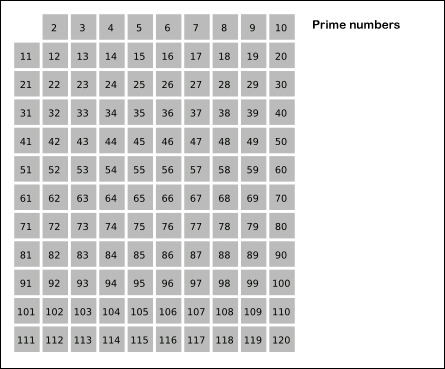
\includegraphics[scale=0.6]{base}
        \item Starting with 2, mark all its multiples, and note 2 as a prime

            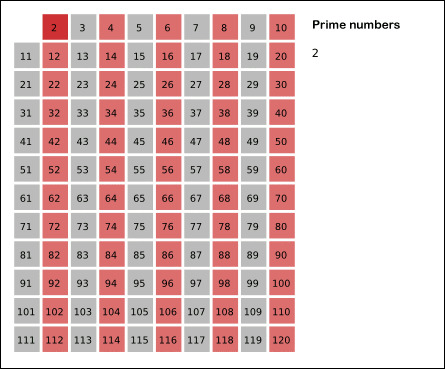
\includegraphics[scale=0.6]{2}\\
        \item Repeat the same process, skipping any marked numbers, and marking
            as prime each unmarked number you encounter

            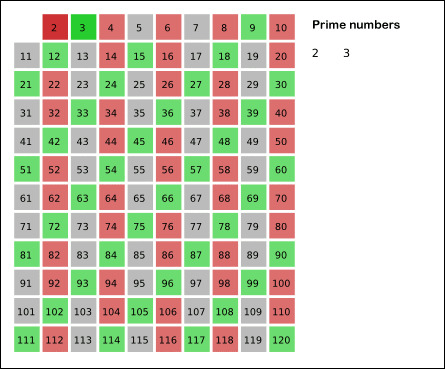
\includegraphics[scale=0.6]{3}\\
            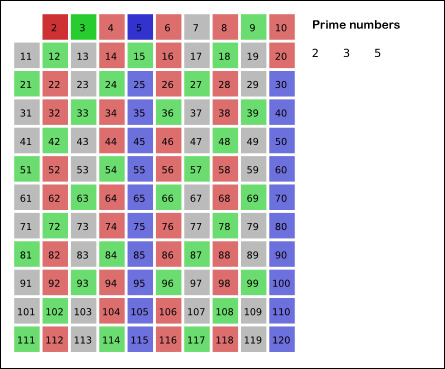
\includegraphics[scale=0.6]{5}\\
            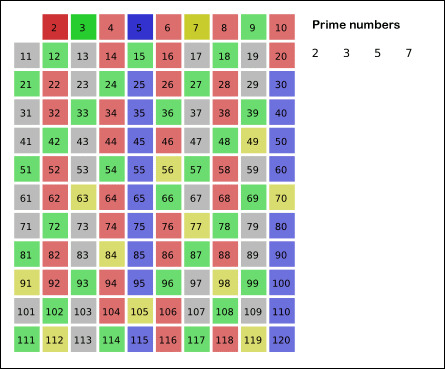
\includegraphics[scale=0.6]{7}\\

    \end{enumerate}

    This method is extremely effective in finding prime numbers, and can even be
    performed by hand for moderately small numbers. However, when applied to
    very large large limits, the method quickly presents a problem of the memory
    required. In order for the sieve to work all found composites must be
    stored, so that they can be skipped. The memory space required for the
    algorithm increases with the limit set, making it impractical for computing
    very large primes.

    \subsection{Fermat's  Little Theorem}
    Fermat's theorem (not to be confused with Fermat's \emph{last} theorem, its
    better known big brother) states that:
    \begin{theorem}[Fermat's Little Theorem]
        $p$ is prime and $p \not|\ a$ $\implies a^{p-1} \equiv 1 \pmod{p}$
    \end{theorem}

    \begin{proof}
        Consider the numbers 0, 1a, 2a, ..., (p-1)a\\
        Suppose two of them $ka,\ la: 1\leq k < l \leq (p-1)$ are congruent
        modulo $p$, i.e. 
    %
        \begin{align*}
                  ka &\equiv la &\pmod{p}&\\
            \iff  k  &\equiv l  &\pmod{p}&\ \text{since p prime and $p \not| a$}
        \end{align*}
    %
        But the integers in $[0, (p-1)]$ form a complete residue system modulo
        $p$, and  $1 \leq k<l \leq (p-1)$, 
        meaning that $k \not\equiv l \pmod p$. \emph{Contradiction}. Therefore, 
    %
        \begin{equation*}
            ka \not\equiv la \pmod{p}\qquad \forall\ k,l \in [0, (p-1)], k \not= k
        \end{equation*}    
    %
        So, $0...(p-1)a$ are all incongruent to each other and so must be, in
        some order, congruent to the least residue system modulo $p$, i.e.
        $0...(p-1)$
    %
        \begin{align*}
            a(2a)...(p-1)a &\equiv 1\times 2\times 3...\times (p-1) \pmod{p}\\
            a^{p-1}(p-1)!  &\equiv (p-1)!                           \pmod{p}\\
            a^{p-1}        &\equiv 1                                \pmod{p}
        \end{align*}
    \end{proof}
            
    \subsection{Fermat test}
    Based on Fermat's theorem, a primality test can be devised.

    Given an even integer $n$ that we want to test for primality we can check
    whether $a^{n-1} \equiv 1 \pmod{n}$ holds for a number of integers $1<a<n$.
    This test cannot, by itself, prove the primality of a given number. It can,
    however, prove compositeness: if $a^{n-1} \not\equiv 1 \pmod{n}$ then $n$ is
    necessarily composite since Fermat's theorem holds for all primes.

    For example, let us test the number 13 for with the fermat test, using the
    bases 5 and 8 (chosen randomly):
    \begin{align*}
        5^{13-1} = 244140625   \equiv 1 \pmod{13}\\
        8^{13-1} = 68719476736 \equiv 1 \pmod{13}
    \end{align*}
    So, 13 appears to be prime. Further testing with all the bases between 1 and
    13 will confirm that 13 is definitely prime.

    Let's also test the Fermat test on a composite number, such as 15, using the
    base 6
    \begin{align*}
        6^{15-1} = 470184984576 \equiv 6 \pmod{15}
    \end{align*}



\section{RSA encryption}
RSA is currently, one of the most popular encryption systems in the world.
It belongs to a category of encryption systems known as public-private key.
This means, that it allows two users to exchange information securely,
without having to exchange a shared encryption key beforehand, as it would
be required by classical encryption systems such as Caesar or substitution
ciphers. 

The system is based on the theory of congruences, and, specifically, on
Euler's Theorem.

    \subsection{The Euler phi-function}
    This function is necessary for Euler's theorem and, subsequently, RSA
    encryption. The definition of the
    function is quite simple.
    \begin{definition}
        $\phi(n)$ is defined as the \emph{number} of integers less than or equal
        to $n$ that are relatively prime to $n$. By convention, $\phi(1) = 1$.
    \end{definition}
    So, for example, $\phi(10) = 4$, $\phi(25) = 20$.

    A quick conclusion that can be drawn is that, for prime $n$, $\phi(n) = n -
    1$, since all integers less than or equal to $n$, aside from $1$ and $n$
    itself, are relatively prime to $n$.

    \subsection{Euler's Theorem}
    \subsection{Definitions \& Terminology}
    Given here are some terms and definitions that will be used:
    %
    \begin{table}[H]
        \begin{tabular}{ | m{5em} | p{30em} | }
            \hline
            Term      & Definition\\
            \hline
            plaintext & The message that will be encrypted, in \emph{plain
                        text}, i.e. before it is encrypted. Usually represented as $M$\\
            \hline
            ciphertext & The message after it has been encrypted. This is what
                         is sent from one user to the other. Without
                         knowledge of the public and private key it is
                         impossible to recover the plaintext using just the
                         ciphertext. Usually represented as $C$\\
            \hline
        \end{tabular}
    \end{table}
    %
    \subsection{Encryption}
    RSA requires a number of values that will be used for the
    encryption/decryption, known as keys.  The first of these are two primes
    $p,q$. These are usually very large numbers, in the order of a few hundred
    or even thousand digits, but for these examples we will use much smaller
    primes, just for the sake of simplicity. Next we assign $n=p \times q$.
    Finally, we need an odd integer $k$ such that $gcd(k, \phi (n)) = 1$ 

    The values we will use for the example are: $p=13$, $q=11$, $n=143 \implies
    \phi (n) = 120$ and $k = 23$

    Let's begin with the encryption of a plaintext message. Firstly, the message
    must be encoded as a number. The simplest way of doing that would be by
    converting character into a number and encrypting each character separately.
    In real world applications, due to the complicated nature of the arbitrary
    messages that have to be transmitted, this encoding cannot be used, but it
    will suffice for this example.

    So, for example, the message "HELLO" would become $08\ 05\ 12\ 12\ 15$,
    using two digits for each character.

    Next, comes the actual encryption. With $C$ as the ciphertext and $M$ as the
    plaintext:
    \begin{equation*}
        C \equiv M^{k} \pmod{n}
    \end{equation*}

    Using the keys we defined, the ciphertext becomes $31\ 18\ 27\ 27\ 24$,
    which can then be safely transmitted, so that it can be decrypted.

    \subsection{Decryption}
    Having received the ciphertext, we can recover the original message using
    the congruence
    \begin{align*}
        M \equiv C^j \pmod{n})\\
        \text{where } kj \equiv 1 \pmod{\phi (n)}
    \end{align*}

    Applying this to our example, we first need to solve $
    kj \equiv 1 \pmod{\phi (n)}$ for j

    \begin{proof}
        Start with the encryption congruence: 
        \begin{align*}
            C & \equiv M^{k} \pmod{n}\\
            M & \equiv C^{\frac{1}{k}} \pmod{n}
        \end{align*}
        We need, therefore, to find $\frac{1}{k} \pmod{n}$, i.e. the
        \emph{multiplicative inverse} of $k$ in modulo $n$. By assumption, 
        \begin{align*}
            gcd(k, \phi (n)) = 1 \\
            \implies \exists\ x: kx \equiv 1 \pmod{\phi (n)}
        \end{align*}
        Let $j$ be a solution to the congruence in the least residue system
        modulo $\phi (n)$ such that $j \in \left[1, \phi (n) \right)$.
        Therefore, $\exists z: kj = z\phi (n) + 1$

        Going back to the encryption congruence we can raise it to the $j^{th}$
        power to get
        \begin{align*}
            C^j & \equiv M^{kj}\\ 
                & \equiv M^{z\phi (n) + 1}\\
                & \equiv M\times M^{z \phi(n)}\\
                & \equiv M\times (M^{\phi (n)})^z\\
                & \equiv M\times 1^z                &\text{(by Euler's theorem)}\\
                & \equiv M \pmod{n}
        \end{align*}
    \end{proof}

\end{document}

